\part{Architecture de l'application} % (fold)
\label{prt:architecture_ _de_ _l_'_application_}
	
	\section{Composants de l'application} % (fold)
	\label{sec:composant_de_l_application}
	\begin{figure}[h!]
			\centering
		    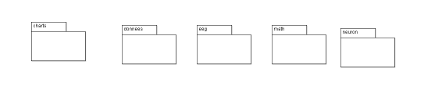
\includegraphics []{../diagramme_classes/packages.png} \\
		    \captionof{figure}{Packages composant l'application}
			\label{fig_pack}
	\end{figure}
	L'application est composée de six packages: eeg, math, neuron, charts, donnees et graphe. Nous allons donc décrire le contenu de chacun de ces packages ainsi que le rôle des classes qui les composent:
	\begin{itemize}
			
	\item [-] eeg : 
		\begin{figure}[h!]
			\centering
		    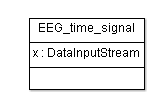
\includegraphics []{../diagramme_classes/eeg.png} \\
		    \captionof{figure}{Classe EEG\_time\_signal}
			\label{fig_eeg}
  		\end{figure}
	 contient la classe EEG\_time\_signal qui contiendra les fonctions concernant le traitement du signal en fonction des données reçues et traitées;
	\item [-] math :
		\begin{figure}[h!]
			\centering
		    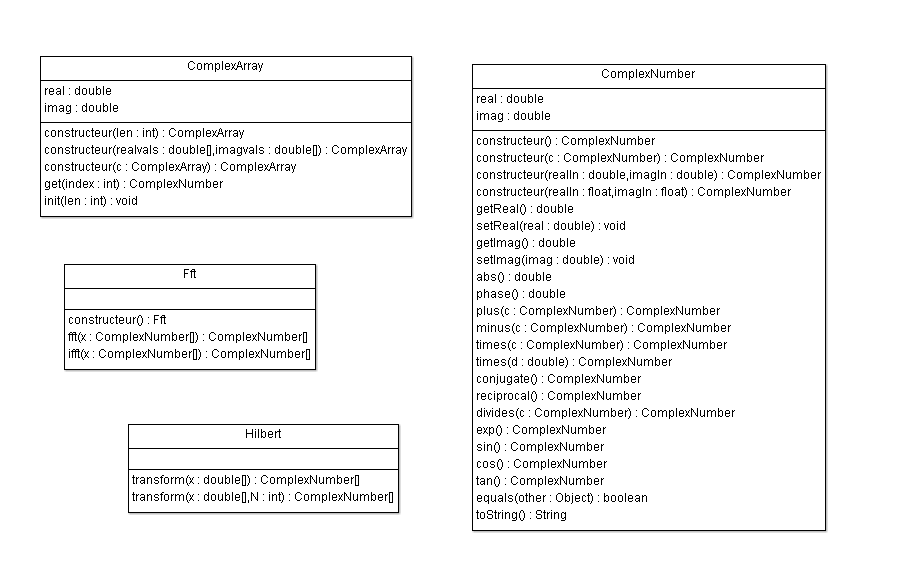
\includegraphics [scale=0.5]{../diagramme_classes/math.png} 
		    \captionof{figure}{Classes pour les calculs mathématiques }
			\label{fig_math}
    		\end{figure} 
	contient toutes les fonctions mathématiques avec la classe ComplexNumber permettant de créer et gérer les nombres complexes, la classe ComplexArray qui permet de stocker les valeurs réelles et imaginaires des nombres complexes, la classe Hilbert qui contient les fonctions concernant les espaces d'Hilbert (extension des espaces euclidiens à des dimensions finies quelconques ou infinies) et enfin la classe Fft qui contient les fonctions en rapport avec la Transformée Rapide de Fourrier(ou Fast Fourrier Transform);
	\newpage
	\item [-] neuron : 
	\begin{figure}[h!]
			\centering
		    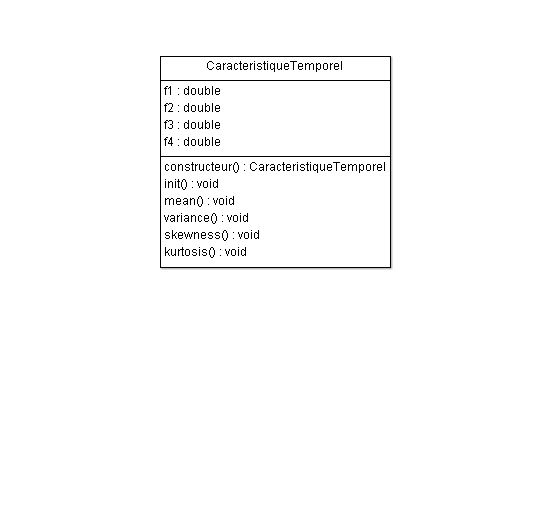
\includegraphics []{../diagramme_classes/neuron.png} \\
		    \captionof{figure}{Classes concernant le réseau de neurones, son apprentissage et ses résultats grâce aux données fournies}
			\label{fig_neuron}
    		\end{figure}
	contient la classe CaracteristiqueTemporel qui contient toutes les fonctions ayant attrait aux caractéristiques temporelles d'un neurone pour le réseau qui sera par la suite créé. Ces caractéristiques temporelles regroupent notamment la moyenne des données, la variance, etc...;
	contient également la classe neuron qui définit les caractéristiques d'un neurone: possède une valeur, une valeur, une donnée des fichiers fournis et un gradient d'erreur qui doit être de 0 lorsque la réponse donnée par le réseau est bonne est bonne;
	la classe LongueurDifferenceException permet de gérer les différences de taille des tableaux passés en paramètres concernant les fonctions appelées dans la classe NeuronNetwork;
	la classe NeuronNetwork représente la constitution et la forme (graphe) du réseau de neurones;
	la classe NeuronNetworkLearnAndResults, quant à elle, permet de tester notre réseau de neurones sur les fichiers de données fournies.
	\item [-] charts :
	 \begin{figure}[h!]
			\centering
		    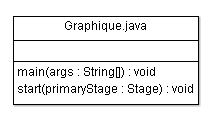
\includegraphics []{../diagramme_classes/charts.png} \\
		    \captionof{figure}{Classe Graphique}
			\label{fig_graph}
			\end{figure}
	 contient la clase Graphique qui permet de tester l'affichage d'un graphique représentant l'un des signaux d'un des fichiers de données fournies grâce à la librairie Open Source java JFreeCharts.
	\item [-] donnees : 
		\begin{figure}[h!]
		    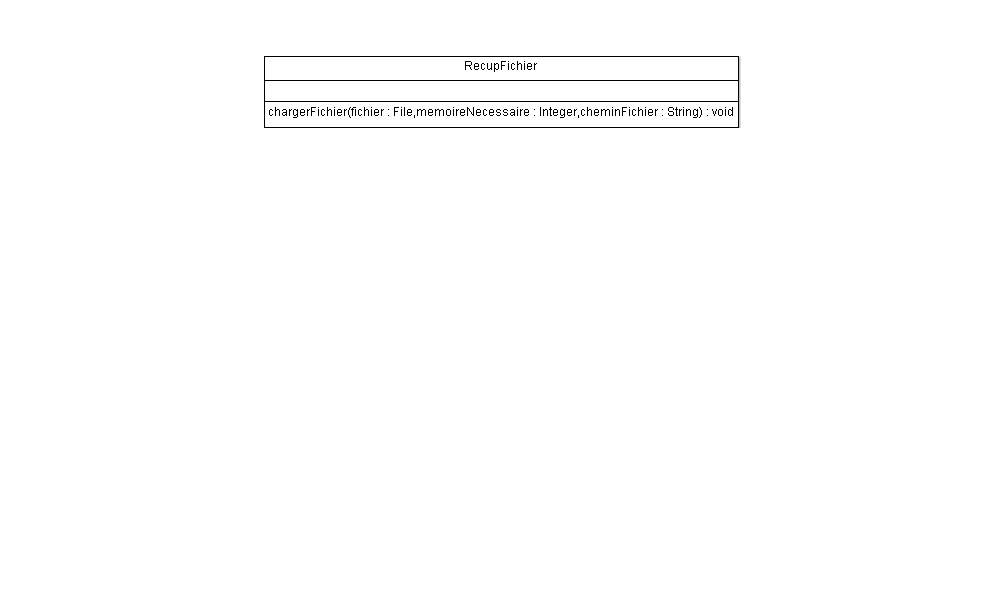
\includegraphics []{../diagramme_classes/donnees.png} \\
		    \captionof{figure}{Classe LireCVS}
			\label{fig_donnees}
  			\end{figure}
	contient la classe LireCVS permettant de récupérer un ou des signaux des fichiers de données fournis pour les stocker en mémoire afin de pouvoir travailler avec.
	
	\item [-] graphe :
	    \begin[figure][h!]
	        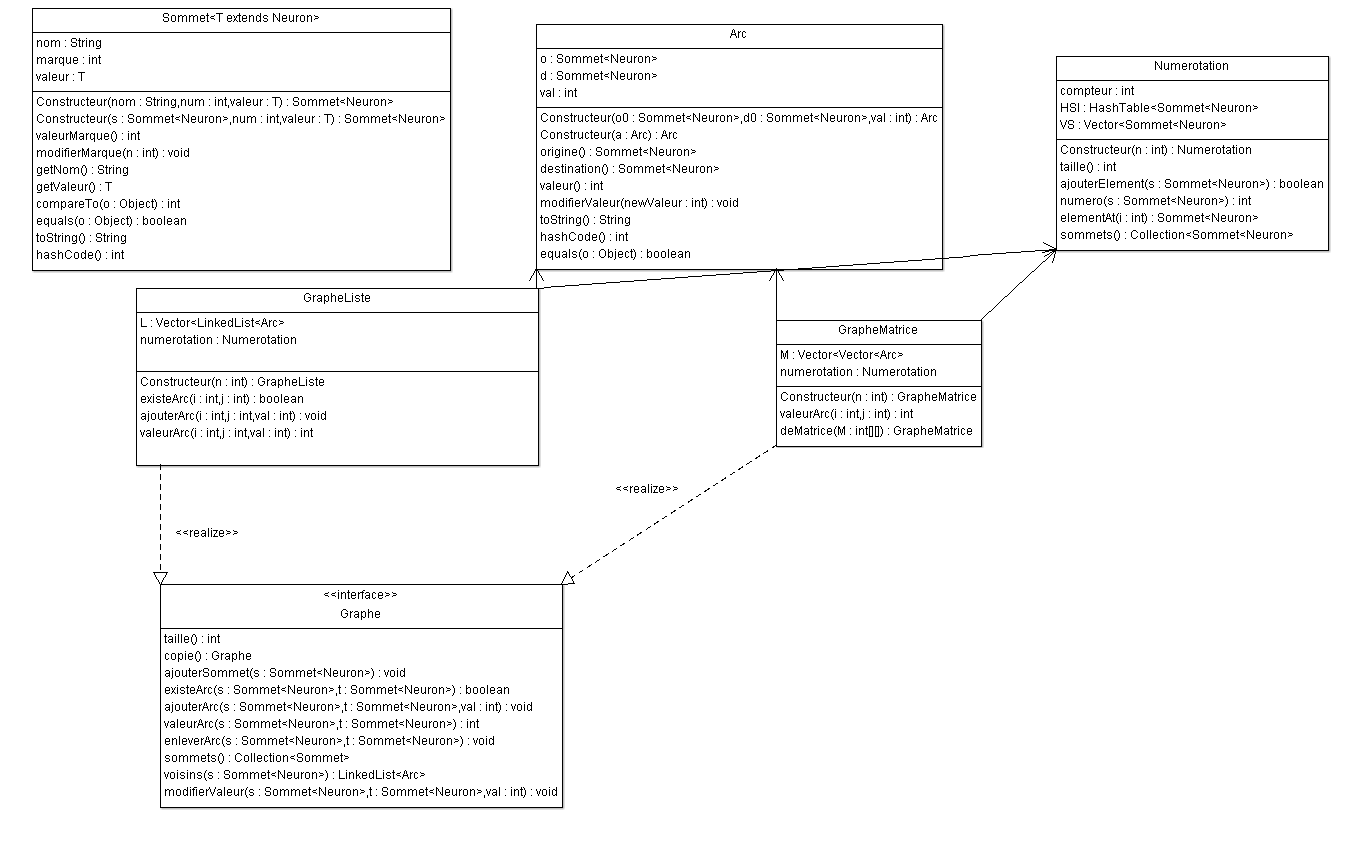
\includegraphics []{../diagramme_classes/graphe.png} \\
	        \captionof{figure}{Classes permettant de définir la forme et la constitution du réseau de neurones}
	        \label{fig_graphe}
	        \end{figure}
	contient les classes permettant de définir la structure du réseau de neurones sous forme de graphe (sommet, arc, forme du graphe, etc...)

	\end{itemize}
	
	% section composant_de_l_application (end)

	\section{Explication Technique} % (fold)
	\label{sec:explication_technique}
		
		\section{Idéés} % (fold)
		\label{sec:idees}

		
		Nous avons eu l'idée, pour ce projet, de créer un "classifieur" représenté par un réseau de neurones afin d'obtenir des résultats à partir d'un flux de données que nous stockerons en mémoire dans un tableau. Chaque donnée sera représentée par un vecteur. Pour chaque vecteur, chacune de ses dimensions représentera une caractéristique du signal EEG du sujet que nous chercherons à reconnaître (le tout afin de reconnaître les états tels : lecture, repos, regarder un film, etc...). Nous sommes partis de ces idées là car, lors de nos lectures sur les interfaces cerveau-machine, il s'est avéré que ce mode de traitement du signal est très utilisé .
		
		% section idéés (end)
		\section{Outils} % (fold)
		\label{sec:outils}
		
		Nous avons développé notre application au moyen du langage Java et nous avons utilisé l'IDE Intellij qui est très pratique car très ergonomique et très intuitif. 
		De plus nous avons utilisé Git comme gestionnaire de versions, le code étant hébergé sur les serveurs de Github. De surcroît, nous avons utilisé JavaDoc pour générer une documentation du code.
		Par ailleurs, nous avons inclus la librairie JFreeCharts pour réaliser des graphiques sans les contraintes de la bibliothèque Swing pour créer des interfaces.Nous avons LaTex afin de rédiger plus facilement nos rapports .
		Par ailleurs, nous avons utilisé le logiciel argoUML pour réaliser le diagramme de classes de l'application et OpenOffice Draw pour réaliser l'organigramme.
		
		% section outils (end)
		\section{Algorithmes} % (fold)
		\label{sec:algorithmes}
		 Par rapport à notre avancement courant, les algorithmes les plus intéressants à présenter sont la fft\footnote{Fast Fourrier Transform} et la transformée de Hilbert qui utilise la fft . \\ 
		 La fft est un algorithme de calcul de la transformation de Fourrier discrète il nous sert lors de la partie de post-traitement du signal, mais aussi dans la transformée d'Hilbert.\\
		 La transformée d'Hilbert est utilisée dans le traitement du signal pour passer le signal réel dans le domaine complexe d’où la classe ComplexNumber. Cette transformée est utilisée lors des calculs des caractéristiques temporelles .

		% section algorithmes (end)
	% section explication_technique (end)
% part architecture_ _de_ _l_'_application_ (end)